\documentclass[]{interact}
\usepackage{epstopdf}% To incorporate .eps illustrations using PDFLaTeX, etc.
\usepackage{subfigure}% Support for small, `sub' figures and tables
%\usepackage[nolists,tablesfirst]{endfloat}% To `separate' figures and tables from text if required

\usepackage{natbib}
\bibliographystyle{chicago}
\setcitestyle{authoryear,open={(},close={)}}
\renewcommand\bibfont{\fontsize{10}{12}\selectfont}% Bibliography support using natbib.sty

\usepackage{hyperref}
\hypersetup{
    colorlinks=true,
    linkcolor=blue,
    filecolor=magenta,
    urlcolor=blue,
    citecolor=blue,
}

\usepackage{titlesec}
\titleformat*{\section}{\Large\bfseries}
\titleformat*{\subsection}{\large\bfseries}

\usepackage{endnotes}
\let\footnote=\endnote
\usepackage{etoolbox}
\patchcmd{\enoteformat}{1.8em}{0pt}{}{}

\theoremstyle{plain}% Theorem-like structures provided by amsthm.sty
\newtheorem{theorem}{Theorem}[section]
\newtheorem{lemma}[theorem]{Lemma}
\newtheorem{corollary}[theorem]{Corollary}
\newtheorem{proposition}[theorem]{Proposition}

\theoremstyle{definition}
\newtheorem{definition}[theorem]{Definition}
\newtheorem{example}[theorem]{Example}

\theoremstyle{remark}
\newtheorem{remark}{Remark}
\newtheorem{notation}{Notation}

\usepackage{tabularx}
\usepackage{booktabs,caption}
\usepackage{threeparttable}

\usepackage{lscape}
%%%%%%%%%%%%%%%%%%%%%%%%%%%%%%%%%%%%%%%%%%%%%%%%%%

\begin{document}

\articletype{DRAFT MANUSCRIPT}

\title{Replication Survey}

\author{
\name{Peter Kedron\textsuperscript{a,b}\thanks{CONTACT Peter Kedron. Email: peterkedron@ucsb.edu}, Joseph Holler\textsuperscript{d}, and Sarah Bardin\textsuperscript{a,c}}
\affil{\textsuperscript{a} Department of Geography, University of California Santa Barbara, Santa Barbara, California, USA; \textsuperscript{b}School of Geographical Sciences and Urban Planning, Arizona State University, Tempe, Arizona, USA; \textsuperscript{c}Spatial Analysis Research Center (SPARC), Arizona State University, Tempe, Arizona, USA; \textsuperscript{d}Department of Geography, Middlebury College, Middlebury, Vermont, USA}
}

\maketitle

\begin{abstract}
Write Abstract

\end{abstract}

\begin{keywords}
Reproducible Research, Epistemology, Geographic Research Methods
\end{keywords}

%%%%%%%%%%%%%%%%%%%%%%%%%%%%%%%%%%%%%%%%%%%%%%%%%%
\newpage
\section*{Introduction}
Since the 1600s, replication has been a defining characteristic of the scientific method and an essential tool of researchers working to understanding and explain phenomena. 
Broadly defined, a replication study is any study that has at least one outcome that would be considered diagnostic evidence of a claim from prior research \citep{nosek2020}.
More frequently, replication studies are differentiated along axes that distinguish the epistemological function they are intended to serve. 
Replications can be used to assess (1) conclusion, (2) internal, (3) construct, and (4) external validity, or (5) may act as confirmatory tests of an underlying hypothesis \citep[see][]{schmidt2009, gomez2010replications, radder2003, radder2012}. 
While the result of a replication study does not provide conclusive evidence for or against a finding, a well-executed, high-quality replication that recreates the results of an prior study typically increases confidence in that finding \citep{earp2015, nichols2021}. 
When prior results cannot be recreated through replication the claims of the prior study, the data and methods used, and the current understanding of the phenomena may be brought into question \citep{christensen2019, NASEM2019}.

While the number of reproduction and replication studies undertaken in the social and behavioral sciences continues to rise, such studies have not yet become commonplace in geography.
The majority of recent research in the geographic literature on the subject has focused on reproduction over replication, and has emphasized the computational reproducibility of geographic research ahead of other dimensions.
For example, an ongoing reproducibility initiative supported by the Association of Geographic Information Laboratories in Europe annually attempts to reproduce the computational results of submissions to their annual meeting and reports on the accessibility of related data, code, and computational environment \citep{nust2018, ostermann2021}.
A series of reproduction studies led by Kedron and Holler \citep{Kedron2023Beyond, Kedron_Holler_Bardin_Hilgendorf_2022} advance this stream of work by introducing selected variations into the reproduction process to test the sensitivity of results to conceptual and methodological perturbations. 
However, those studies also largely focuses on testing the conclusion and internal validity of past studies through computational reproduction. 

The small number of published studies that have attempted to replicate geographic research suggest that many studies cannot be fully replicated \citep[e.g.,][]{Kedron2022dimaggio, paez2022reproducibility}, or are simply missing components needed to attempt a replication \citep{konkol2019, ostermann2017}.
More often the literature on the replication of geographic research turns to the question of if and when it is reasonable to expect the findings and claims of a prior study to replicate \citep{kedron2021GA, kedron2022replication, goodchild2021replication, sui2021reproducibility}. 
Place to place variation in phenomena, and the processes that produce them, are one of the defining features of geographic research and a central tenant of many of its research traditions.
With those intellectual foundations, it remains unclear how current geographic researchers view replication and its role in the knowledge accumulation process.
There is similarly limited empirical evidence available about the factors that motivate or discourage geographic researchers from pursuing replications. 

To address this gap in our collective knowledge, we surveyed geographic researchers about their understanding of replicability, beliefs about what factors affects the chances or replicating a study, motivations to attempt replication studies, and experiences conducting replications.
We are aware of only a handful of similar published surveys within the geographic literature \citep{balz2020reproducibility, konkol2019, ostermann2017, kedron2023survey}.
However, these surveys typically focus on the quantitative and computational intensive forms of geographic research, primarily assess the availablity of research artifacts (e.g., data and code), and address reproducibility, whether the same results can be created using the same data and methods, rather than replicability. 
In all but one instance, these surveys also rely on convenience samples drawn from specialist conferences or non-representative subsets of the geographic research community. 
In contrast, to support generalization, we designed a sampling frame to capture researchers from across disciplinary subfields and methodological approaches, and draw survey participants from that frame using a probability sampling scheme.
In the remainder of this paper, we detail the design of our survey, sampling strategy, and analytical approach before presenting the results of our survey. 
We then discuss the implications and limitations of our work. 


%%%%%%%%%%%%%%%%%%%%%%%%%%%%%%%%%%%%%%%%%%%%%%%%%%
\section*{Data and Methods}
Complete documentation of the procedures, survey instrument, and other materials used in this study are available through the Survey of Researcher Perceptions of Replication in Geography Repository (\citet{Kedron_Holler_Bardin_Hilgendorf_2022} - \url{https://osf.io/x6qrk/}).
The repository connects to a GitHub repository which hosts the anonymized dataset and code used to create all results and supplemental materials along with a complete history of their development. 
All of the results presented in this paper can be independently reproduced using the materials in that repository.
Before the start of data collection, we registered a preanalysis plan for the survey with OSF Registries (\citet{Kedron_RPl_Survey_PAP} - \url{https://osf.io/a4nwg}). 
The survey was conducted under the approval and supervision of the Arizona State Institutional Review Board - \textit{STUDY00014232}.

%%%%%%%%%%%%%%%%%%%%%%%%
\subsection*{Sampling Frame}
Our target population of interest is researchers who have recently published in the field of geography. 
We followed a 4-step procedure to create a sampling frame for our survey that captures this diverse population of researchers. First, beginning at the publication level, we identified journals indexed as either geography or physical geography by the \href{https://access.clarivate.com/}{Web of Science's Journal Citation Reports} that also had a 5-year impact factor greater than 1.5.
From those journals, we created a database of all articles published between 2017 and 2021.  

Second, we used Arizona State University's institutional subscription to the \href{https://www.scopus.com/home.uri}{Scopus Database} to extract journal information (e.g., subject area, ranking), article information (e.g., abstract, citation counts), and author information (e.g., corresponding status, email) for each publication. 
Because our intention was to capture individuals actively publishing new geographic research, we retained publications indexed by Scopus as \textit{document type = ``Article''} and removed all other publication types (e.g., editorials, book reviews) from our article database. 
We also removed articles with missing authorship information. 

Third, moving to the researcher level, we created a list of researchers and their published articles, focusing on corresponding authors for two reasons.
(1) Corresponding authorship is one indicator of the level of involvement an individual had in a given work. 
While imperfect, it was the best available indicator in the Scopus database as across journals there is no commonly adopted policy for declarations of author work (e.g., CRediT Statements).
(2) Scopus maintains email contact information for all corresponding authors, which gave us a means of contacting researchers in our sampling frame.
Scopus also maintains a unique identifier for each author (author-id) across time, which allowed us to identify authors across publications. 

Fourth, we constructed a sampling frame of unique researchers and their most recent email contact information. 
We determined uniqueness by grouping researchers by their author-id, and we determined the most recent contact information by selecting records associated with the most recent year of publication. 
For 383 researchers who had two or more distinct emails in the latest year of publication, we removed non-institutional personal email addresses and then selected one of the remaining institutional email address.

Applying these criteria yielded a sampling frame of 29,828 researchers. 
On average, these authors published 2.7 articles in geography journals meeting our criteria between 2017 and 2021. 
Roughly one-third (33.0\%) were most recently a corresponding author for an article published in a general geography journal. 
A similar proportion (32.0\%) were most recently a corresponding author for an article published in an earth sciences journal, and smaller proportions had published in the social sciences and cultural geography (20.0\% and 16.0\%, respectively).

\subsection*{Survey Instrument}
The survey first established eligibility based on age and geographic research activity in the past five years and asked researchers to report their primary subfield and methodology.
We asked each participant to assess their familiarity with the term ``replicability'' and to provide their own definition. 
We then provided a definition based on the \citet{nosek2020replication}  to establish a common understanding of replicability for the remainder of the survey.
Remaining questions assessed the epistomological purpose of a replication (5 questions), what portion of the geographic literature has/could/should be replicated (3 questions), and factors that impact the chances of successfully replicating a study (18 questions) or the decision to attempt a replication (13 questions).
For researchers who reported attempting reproductions, we asked them to elaborate on their motivations and outcomes (9 questions).

We developed the survey questions following a review of prior reproducibility surveys \citep[e.g.,][]{fanelli2009many,baker20161, konkol2019} and our own reading of recurring issues in the reproducibility and replicability literature. 
We pilot tested the survey instrument with \textit{n}=15 graduate students and geography faculty with differing levels of experience, topical focus, and methodological background. 
After pilot testing, we removed these individuals from our sampling frame to ensure they would not be included in our final sample.

%%%%%%%%%%%%%%%%%%%%%%%%
\subsection*{Data Collection}
We used a digital form of the Tailored Design Method \citep{dillman2014internet} to survey geographic researchers between Oct 3 and Oct 27, 2022.
A simple random sample of 2,000 researchers was drawn without replacement from our sampling frame, and those researchers were invited via email to participate in the online survey. 
Researchers received their initial invitation on Oct 3, 2022. 
Two reminder emails were sent to researchers that had not yet completed the survey on Oct 13 and Oct 20, 2022.

The online survey was administered through \href{https://www.qualtrics.com/}{Qualtrics}. 
Participation in the survey was entirely voluntary. 
Each researcher that opted to participate in the survey was provided with IRB approved consent documentation and linked to the internet survey instrument. 
Participants were also given the option to provide an email address for eligibility for one of three  prizes of 90 US\$, selected randomly after the data collection period.
Participating researchers had the option to exit and re-enter the survey and were also able to review and change their answers using a back button as they progressed through the survey.
At the end of the data collection period, responses were checked for completeness and coded using the reporting standards of the American Association For Public Opinion Research \citep{aaporstandards}.
Responses were downloaded from Qualtrics, anonymized, and stored in a public de-identified database in the research compendium.

%%%%%%%%%%%%%%%%%%%%%%%%
\subsection*{Analytical Approach}

We conducted two analyses of the survey responses.
First, we analyzed researcher perspectives on replicability by coding and calculating summary variables and statistics for three themes: how geographic researchers define replicability, factors researchers believe affect the chances of replicating a study, and factors researchers believe affect the decision to attempt to replicate a study.
Second, we analyzed the experiences of researchers attempting to replicate prior studies using statistical summaries of participant motivations, research practices, and ability to recreate study results.
For both analyses, we produced and analyzed descriptive statistical summaries of participant responses to Likert scale questions cross-tabulated by disciplinary subfield and methodological approach.
For free-from text responses we coded responses and selected illustrative examples for inclusion. 

For free-form text definitions of ``replicability'' we coded participant responses using two procedures. 
First, we measured the similarity of each provided definition to the definition adopted by the \citet{NASEM2019}. 
The NASEM defines reproducible research as having three characteristics --- new data, same procedure, and same or similar results.
To make this comparison, two of the authors independently coded each respondent definition for the presence/absence of each of these the three characteristics.
Disagreements in the assignment of codes were resolved through discussion between the three authors.
We created an aggregate measure of definition similarity for the final coded response for each participant by counting the presence of each NASEM definition characteristic, resulting in a measure with the domain [0, 3].

Second, we coded each definition to identify mentions of: (i) internal validity assessment, (ii) external validity assessment, (iii) the significance of spatial or temporal context, (iv) epistemological necessity, and (v) adherence to open science practice.
We derived this coding from common themes in the responses and our own reading of the replicability literature.
As above, each definition was independently coded by each author before code assignments across authors were compared with disagreements resolved through discussion.
Our first set of analyses examined the full set of survey responses, while our second set of analyses were restricted to the 84 participants that reported attempting a replication study in the past two years.

%%%%%%%%%%%%%%%%%%%%%%%%%%%%%%%%%%%%%%%%%%%%%%%%%%
\section*{Results}
A total of \textit{n}=283 of the authors we contacted completed the online survey with information sufficient for analysis. 
The contact rate for the survey was 18.8 percent, the response rate was 14.1 percent, yielding a cooperation rate of 74.4 percent. 
The refusal rate was 4.8 percent\endnote{All outcome rates are reported using \citet{aaporstandards} standards. 
The outcome rates used were - response rate 2, cooperation rate 2, refusal rate 1, and contact rate 1.}.
Respondents were predominantly male (65.1\%) and between the ages of 35 and 55 (62.4\%). 
The majority of respondents were also academics, but were well balanced across career levels as no one category made up more that 30 percent of the sample.
Respondents were similarly balanced across disciplinary subfields, but did contain a greater number of physical geographers  - human geography (26.8\%), physical geography (39.9\%), nature and society (14.8\%), geographic methods and GIScience (17.3\%). 
Different methodological approaches were well represented by respondents in the sample with qualitative researchers making up the smallest sub-group  - quantitative (47.3\%), qualitative (16.3\%), and mixed-methods (36.0\%).

%%%%%%%%%%%%%%%%%%%%%%%%
\subsection*{Researcher Definitions of Replication and its Epistemic Functions}
Geographic researchers are thinking about replicability and link the act of replicating a study to a number of different epistemological functions (Figure \ref{fig:Q7-Epistemology}). 
A majority of respondents reported thinking about replicability (74\%), talking with colleagues about replicability (65\%), and considering replicability when undertaking peer-review (59\%) during the past two years. 
In particular, respondents believe that replication studies can be used to assess the construct validity (75\%) and external validity of a prior study.
Specifically, respondents believe that replication studies can assess whether the claims of that study will hold in new locations (67\%) or new populations (63\%). 
While respondents clearly linked replication to epistemological functions, across all functions they were more likely to agree than strongly agree that replications could serve these purposes.
Respondents that identified as human geographers or as studying nature and society were less likely to agree that replications could be used to achieve these goals when compared to those working in other subfields. 
For example, 87 percent of respondents specializing in GIScience and methods believe replications could be used to assess whether a claim was the product of chance, compared to just 57 percent of human and nature-society researchers.

\begin{center}
\textbf{Insert Figure \ref{fig:Q7-Epistemology} About Here}
\end{center}

While respondents largely agree that replication has some epistemological role to play in the geographic research process, many respondents did not explicitly include these same concepts in their definitions of replicability.
At total of 253 of our respondents provided an interpretable definition of replicability, but only 68 of those definitions (26\%) referenced some form of epistemological function. 
Using replication to externally validate the claims of a study was identified by 49 respondents (19\%).
No other epistemological function was mentioned by more than 13 respondents (5\%).  
In contrast, 123 respondents (48\%) reported that replications could be used to o assess or improve how well a prior study conforms to the principles of open science.

Rather than focusing on these larger concepts, most respondents used their definitions to present the criteria that identify a study as a replication.
On average, respondents provided definitions that included 1.2 of the three characteristics of the replicability definitions adopted by the NASEM.
Comparing the similarity of results between studies (65\%) and using the same method across studies (56\%) were the characteristics of replicability most frequently identified by respondents.
Less than a quarter of respondents explicitly included use of the collection of new data (12\%) in their definitions.
Only seven percent of respondent definitions included all three characteristics identified by the NASEM.
The pattern of similarity to the NASEM definition and each of its components was consistent across subfields and methodological approaches, with a slightly greater emphasis placed on methodological consistency by quantitative and geographic methods and GIS researchers.

Respondents specializing in different subfields and methodological approaches also emphasized different epistemological roles for replication in the research process.
For example, on \textcolor{red}{INSERT SOME CONTRASTING QUOTED EXAMPLES HERE.}

%%%%%%%%%%%%%%%%%%%%%%%%
\subsection*{Factors Affecting the Chances of Replicating a Prior Study}
Overall respondents believe that the majority of research in the discipline has not been independently replicated and appear to be uncertain about what proportion of the literature could or should be replicated (Figure \ref{fig:Q12-HCS}). 
On average, respondents estimated that 25 percent of recent studies in their sub-field have be replicated. 
However, the distribution of these responses is strongly right skewed.
In fact, 47 percent of respondents estimated that less than 10 percent of recent studies have been replicated.
It is similarly unclear if respondents believe recent geographic research could or should be replicated.
On average, respondents estimated that approximately half of studies 'could be replicated' (55.0\%) or 'should be replicated' (55.9\%). However, the distribution of responses to both questions are relatively flat across the range of possible values and highly variable (\textit{$sd_{could}=24.3\%$}, \textit{$sd_{should}=27.7\%$}), which suggests 
respondents were uncertain whether it was possible or valuable to replicate recent research.  

\begin{center}
\textbf{Insert Figure \ref{fig:Q12-HCS} About Here}
\end{center}

Respondents identified a range of factors that might impact the chances of an independent researcher replicating the claims of a prior study (Figure \ref{fig:Q8-10-Chances}a).
A majority of respondents identified the transparency and availability of the components of a study as affecting the odds of replication. 
Poor documentation of the original study (75\%) and the use of restricted access data (66\%) were seen by the greatest number of respondents as decreasing the odds of being able to replicate a prior result. 
Some respondents identified the inclusion of multiple sites in a study as increasing the chances of an independent replication of the findings of that study (39\%), but not in great enough numbers to constitute a majority. 

The characteristics of the research team that conducted the original study were generally not identified by respondents as likely to change the changes of replicating that study. 
The majority of respondents (51\%) indicated that a large research team working on the prior study would have no effect on the chances of an independent researcher replicating that work. 
The remaining respondents were nearly evenly split as to whether a large team would increase of decrease the chances of replicating that study. 
On the whole, more respondents believed that reliance on the unique expertise of the research team conducting a study, or the position adopted by that team would decrease, rather than increase, the chances of replicating the claims of a study.
However, only 53 percent of respondents thought the position a research team chose to adopt when conducting study would decrease the chances of replicating that study. 
Similarly, 48 percent of respondents identified reliance on the unique expertise of the original researcher team as decreasing the odds of replicating a study. 
In both cases, 24 percent of respondents reported that they did not believe either factor would impact the odds of replicating a prior result.

Respondents were similarly divided about the extend to which the approach adopted in the prior study would affect the chances of replicating that study. 
Respondents were nearly evenly split as to whether the number of hypotheses tested by a study, and whether that study used qualitative or mixed methods would increase or decrease an independent researcher's chances of finding results that supported the claims of the prior study.
About a quarter of respondents said that use of a mixed methods approach or the testing of multiple hypotheses had no effect on the chances of replication.
In contrast, a large majority (80\%) of respondents identified the use of quantitative methods in a prior study as increasing the chances of replicating that study. 
This result matches the association observed in respondent definitions of replication, which ties replication to positivist science and quantitative approaches to knowledge creation.   

\begin{center}
\textbf{Insert Figure \ref{fig:Q8-10-Chances} About Here}
\end{center}

There was less agreement among respondents about whether different characteristics of a phenomenon would impact the chances of replicating the claims made by a prior study of that phenomenon (Figure \ref{fig:Q8-10-Chances}b). 
For all six of the characteristics we examined, at least 12 percent of respondents replied that those factors would have no effect on the chances of replicating a prior study.
Numerous respondents also replied that they the simply did not know whether a characteristic would impact the chances of replicating a study. 
For example, 20 percent of respondents said they did not know whether a phenomenon being spatially dependent with itself would affect the chances of replicating a prior study, and an additional 15 percent of respondents said spatial dependence would have no effect on replication. 
Even with this uncertainty, 41 percent of respondents said the presence of spatial dependence was likely to decrease the chances of replicating a prior study.

A majority of respondents did identify the inability to directly measure a phenomenon (61.5\%) and a strong relationship between a phenomenon and local conditions (59.7\%) as reducing the chances of replicating a prior study.
Respondents were roughly evenly divided on whether other factors would increase or decrease the chances of replicating a study.
Respondents also favored 'somewhat likely' responses over stronger 'very likely' responses across all characteristics, which further suggests that absence of a clear consensus understanding of how these factors relate to and impact replication.


%%%%%%%%%%%%%%%%%%%%%%%%
\subsection*{Factors that Affect the Decision to Attempt Replications}
Several factors appear to affect whether researchers decide to attempt to replicate recent geographic research (Figure \ref{fig:Q15-DecisionFactors}).
Geographic researchers identified current academic incentives as the factor most frequently impacting the decision to attempt a replication study. 
A majority of respondents identified the pressure to publish original research (66\%) and the lack of funding for replication studies (59\%) as frequently or always impacting the decision to attempt a replication.
Respondents also believed that the perception of replications as low value work (55\%) that was often difficult to publish (51\%) also impacted decision making.  
Contrary to some narratives in the replication literature, the desire to identify fabricated data or results was not seen as a determining factor in the decision to attempt a replication. 
However, this finding should be interpreted with caution as a third of respondents indicated that they did not know whether potential fabrication influenced researcher decision making.  

\begin{center}
\textbf{Insert Figure \ref{fig:Q15-DecisionFactors} About Here}
\end{center}

Respondents also identified the availability of research artifacts as important to the decision to attempt a replication study.
Respondents believe that difficulty accessing and recreating data (54\%) frequently or always affects the replication decision.
Similarly, respondents (45\%) identified the accessibility of procedural and methodological information as a influential factor. 
The challenge of recreating the methods of a prior study elicited a similar response (41\%).

No characteristics of the original study, or the potential replication attempt, were identified by a majority of researchers as frequently or always impacting the replication decision. 
However, some respondents did identify inexperience conducting replication studies (37\%) and potential geographic variation in the phenomena being investigated (33\%) as always or frequently influencing decisions to attempt replications. 
Moreover, many respondents also saw these factors as occasionally affecting the decision to attempt a replication.
Few respondents see a low chance of successfully replicating a study as a deterrent to attempting a replication, but it is unclear whether this result is driven by a belief in the value of null replication results, or the belief that replications have high chances of success.
Finally, respondents did not identify ethical concerns as a factor affecting the decision to attempt a replication study. 
However, several of these results should also be interpreted with caution. 
More that 15 percent of respondents replied that they did not know whether geographic variation, inexperience with replication, or ethical concerns would affect a researcher's decision to attempt a replication. 

Respondents also identified a number of factors that were omitted from our survey instrument as important when deciding whether to attempt a replication of a geographic study. 
These factors include practical issues such as the difficulty identifying and accessing new field sites where data would be collected during a replication attempt, the costs of conducting a replication, and the time needed to obtain institutional approvals.
Respondents also identified uncertainty about how to compare the results of a replication attempt to the original as important when deciding to undertake a replication attempt. 
Finally, a small number of respondents believe that geographic researchers do not undertake replication studies because they either believe that replication is not possible or not necessary in geography. 
These respondents argued that the main value of geographic studies is that each study provide a unique lens on the portion of the world under investigation, which makes replication a unnecessary endeavour.   

Respondents from different disciplinary sub-fields and methodological approaches varied little in their identification of the factors affecting researchers' decisions to attempt replication studies (Table \ref{tab:motivations}). 
Human geographers and researchers using quantitative methods less frequently identified academic incentives as important to the replication decision when compared to other sub-groups, but were otherwise broadly similar in their views on artifact availability and study characteristics. 
A greater percentage of quantitative researchers and those working in the areas of GIScience and Methods identified the accessibility of data and methodological information as more often impacting the decision to replicate, but not at a level that was substantially higher than other sub-groups. 
In fact, a greater percentage of researchers studying nature and society identified data accessibility as important than did methods researchers.  

\begin{center}
\textbf{Insert Table \ref{tab:motivations} About Here}
\end{center}

%%%%%%%%%%%%%%%%%%%%%%%%
\subsection*{Replication Attempts}
In total, 84 of the researchers that responded to our survey (30\%) reported attempting to independently replicate at least one study in the last two years.   
This subset of participants formed the basis for our analysis of researcher experiences when attempting to replicate of the work of others.
Respondents specializing in physical geography made up the greatest percentage of replication attempts, but researchers from all the subfields we examined reported attempting replication studies - physical (39\%), human (24\%), GIScience and methods (19\%) and nature and society (15\%).  
Respondents attempting replications predominantly focused on quantitative (52\%) and mixed-methods (37\%) research designs. 

Most respondents reported that their replication studies were conducted in locations that differed from those of the original study (50\%), or that they first attempted to recreate the results of the original study in the same location before also testing them in a new location (18\%). 
Of the 47 respondents that identified why they decided to attempt their replication study, 38 reported they were attempting to externally validate the claims of the original study, while 20 percent reported that they were motivated to examine the impact a difference in geographic or temporal context might have on the results. 
For example, \textcolor{red}{PULL EXAMPLES FROM Q19}.
A total of 16 respondents also identified replication as a fundamental part of knowledge creation and evaluation. 
For example, \textcolor{red}{PULL ONE EXAMPLE FROM Q19}.

In the majority of the attempted replications, respondents reported that they were able to recreate at least some of the results of the study they were investigating and form conclusions that matched those of the original study from those results. 
55 respondents (62\%) reported being able to exactly replicate some of the results of a prior study. 
However, only six respondents (7\%) reported that they were able to exactly replicate all results.
The survey results were similar when we asked respondents whether they were able to partially replicate the results of a study --- finding a different result, but ultimately coming to a similar conclusion as the prior study. 
62 respondents (73\%) reported being able to partially replicate at least some of the results of a study, while 14 respondents (16\%) reported being able to partially replicate all results. 

Respondents reported a limited ability to access the data, code, and procedures used in the studies they were attempting to replicate. 
Respondents were generally able to access some (51\%) or all (31\%) of the data used in a prior study, but were slightly less successful at accessing some (42\%) or all (28\%) of the code and procedural information.
Moreover, being able to access these materials and information did not mean that researcher could fully understand or directly replicate how a study was conducted.
Only 16 respondents that attempted replications (19\%) reported being able to follow all of the procedures of a prior study without having to make additional assumptions about how the procedure was implemented. 
In all other cases the replicating researcher had to make additional assumptions about how the authors of the original study conducted their work.
Respondents also reported that their replication attempts where complicated by an inability to recreate the computational environments of prior analyses and the unavailability of details about where a prior study was conducted.
In only 31 cases (37\%) was the researcher able to find complete details about the geographic extent and location of the prior study.

Ultimately 58 respondents that attempted replications (69\%) reported publishing some or all of their findings.
23 respondents were able to publish all of the findings of their replication study, while another 36 respondents were able publish at lest some of their findings.
48 Respondents that either did not attempt to publish their findings, or were only able to publish a portion of their findings, reported why they chose not to attempt publication. 
27 respondents replied that replications were still ongoing or that it would simply take too much time to pursue publication. 
Many other respondents said that they believe it would either be to difficult to publish their replication study because replications were not valued in the academic literature.
For example researchers pointed out that, "no one seems to care", their results received "no interest from journals", and that "incentives in academia clearly point towards publishing original research."
In one instance, "The journal that published the original paper specifically claimed to be interested in replications, but then desk rejected our replication."
This reasoning reflects different form of non-response and selection bias at the root of the 'file drawer problem' in academic literature (CITE - Rosenthal 1979). 
The file drawer problem exists when the outcome of a study influence the decision to publish or share that finding. 

%%%%%%%%%%%%%%%%%%%%%%%%%%%%%%%%%%%%%%%%%%%%%%%%%%
\section*{Discussion and conclusion}
The results of our survey suggest geographic researchers are familiar with replication and believe that replication studies can serve several epistemological functions.
However, we also found that researcher provided definitions often did not clearly articulate the epistemological role, or roles, that could be played by a replication study. 
Researcher definitions instead focused on criteria used to identify a study as a replication. 
This same focus on criteria can be observed in the wider R\&R literature, where authors typically broadly gesture to the epistemological function of replication then quickly turn to the accounting of data and code sharing practices. 
This tendency toward criteria suggests that replication as an epistemological tool may not be at the forefront of geographic researchers' thinking about replication.

It also remains unclear if or how geographic researchers map variations between an original study and its replication to the epistemological functions that replication study is intended to serve.
A clear understanding of this connection between variations and functions is essential because which aspects of a study are changed controls the form of validity being assessed \citep{gomez2010replications, radder2003, schmidt2009}.
Poor documentation and articulation of these connections in replication studies of geographic research could lead to the misinterpretation of the results of an individual replication, and could misdirect the collective assessment of a claim across a set of replication studies.
Developing a schema to map replication study variations to functions may be particularly challenging in geography due to the complexity of geographic systems and the limited control researchers have over those systems. 
Moreover, it is often unclear which aspect of a study are changing when a replication study is conducted in a new location. 
For example, when a researcher conducting a replication collects new data from a new location it may be difficult to determine whether the study is testing the external validity of a claim in a new population, or in the same population that is subjected to different place-based processes.
Our results suggest that a conceptual treatment of these connections attuned to the peculiarities of spatial data analysis would be an important first step toward conducting and systematically assessing interpretable replication studies of geographic research. 

The results of our survey suggest that collectively researchers are uncertain whether it is valuable to replicate recent geographic research. 
Our results do indicate that it is unlikely that this uncertainty stems from a lack of belief in the potential epistemological value of replication studies.
Instead, mirroring traditional debates within the discipline, it may be the case that researchers are uncertain whether, or to what extend, the results and claims of a study should be expected to replicate in new locations. 
Researcher uncertainty may also be a reflection of the perceived quality and importance of the available geographic literature. 
If researchers believe many studies simply do not contain important findings, it would be rationale not to prioritize replicating those studies.
Finally, researchers may simply perceive the external validity check offered by replication as not important to the goals of their research tradition. 
Following \citet{sayer1992method} distinction between intensive and extensive research, many traditions in geography focus on reconstructing the causal chains that structure social and environmental relations in specfic contexts, rather than the discovery of empirical regularities across those contexts. 
While some of the qualitative responses to our survey are suggestive of these points, follow-up research could delve more deeply into which studies researcher believe are valuable to replicate and why.

Disciplinary variation
\begin{itemize}
    \item Overall, the differences we observed across sub-groups was small, but should be interpreted with caution given the sub-group sample sizes.
    \item We also found that human geographers and qualitative researchers were disproportionately likely to provide 'I do not know' responses across questions, which further decreases the amount of information available about their views and beliefs. 
\end{itemize}

%%%%%%%%%%%%%%%%%%%%%%%%
\subsection*{Limitations} 
Survey research has several common limitations which we attempted to mitigate through the design of our study. 
Unlike prior surveys of reproducibility and replicability, our study uses a sampling frame designed to be representative of our target population of active geographic researchers. 
However, use of a well-constructed sampling frame and probability sampling do not ensure that a balanced and representative sample will be drawn from the target population. 
Ideally, we would stratify our potential respondents into meaningful subgroups, randomly draw participants from these subgroups, and use a post-stratification procedure to address any imbalance in our response. 
However, we could not follow this approach because stratification require knowledge of the population characteristics that predicts differences in response and a population wide census of those key predictors.
We did not have access to this information because we presently lack a comprehensive understanding of replicability in geography and no list of geographic researchers complete with relevant predictor information exists.
Given these limitations, our study should be viewed as an exploratory analysis with random sampling and a transparent, reproducible methodology for sample frame construction.

We have similarly worked to reduce the effects of several other common forms of bias from our survey.
We have worked to eliminate exclusion bias by including in our sampling frame all researchers publishing as corresponding authors in any wide range of geography journals over a five year period.
However, geographic researchers publish in a range of journals that are not necessarily indexed as geography by the Web of Science. 
Geographic researchers that have only published outside geographically indexed journals would not be captured in our sampling frame which would create exclusion errors. 
However, we believe the number of individuals falling into this category will be small as most active geographic researchers are likely to have published at least one study in the journals meeting our inclusion criteria.

Similarly, we cannot eliminate the possibility of self-selection bias from our survey. 
It may be the case that geographic researchers more familiar with replication, or those working in subfields more involved with current R\&R debates (e.g., quantitative, computational research) were more likely to respond to our survey. 
Conversely, it may also be the case that researchers working in subfields traditionally associated with critiques of a positivist scientific approach (e.g., qualitative, human geography) were less likely to participate in our survey. 
We attempted to quantify potential self-selection by calculating and comparing survey completion rates across subfields and approaches. 
Completion rates for all subfields were between 84 and 87 percent, except slightly higher rates for geographic methods and GIS researchers (96.8\%).
Completion rates were 84.2 percent for mixed methods, 87.0 percent for qualitative methods, and 91.1 percent for quantitative methods. 
These values suggest that self-selection was not a significant issue.

We attempted to mitigate the potential for questionnaire bias, which could be caused by partially basing our survey instrument on prior studies that over-represent perspectives from the computational and experimental sciences.
If this were the case, our survey may not gather data on researcher practices and beliefs relevant to replicating types of research not well represented in the existing literature. 
To address this concern, we incorporated into our survey instrument questions informed by a parallel review of the R\&R literature available within geography and a review of critiques of positivist science made by social scientists and human geographers.
We also provided the option for an open ended text response to questions to identify issues we did not anticipate during instrument construction.  

Finally, our survey provides a description of the perspectives of geographic researchers at one point in time and one depth of understanding.
As the first survey of its kind, our work provides an initial measurement of geographers definitions of replicability, beliefs about what factors affects the chances
or replicating a study, motivations to attempt replication studies, and experiences
conducting replications. 
However, in many cases we were not able to probe more deeply into the nuances of these measurements and the conceptualization that underlie them.
For example, as highlighted in the discussion, we were able to gain only limited insight into the epistemological roles researchers believe replications can serve and how they map those roles onto what is changes in a replication study.
Future research using in-depth interviews or multi-analyst study designs could probe these question more deeply. 
It would also be useful to track the information collected in this survey over time and to link that tracking to specific topics. 
For example, understanding how researcher perspectives on the epistemological function of replication shift in climate change impacts research may be a useful indicator of how well researchers in that field are developing theories and methodologies capable of dealing with increasing variation and shifting baselines induced by climate change.
More broadly, regular monitoring of perceptions of replication would help identify areas in need of engagement, as well as the success or failure of past investments designed to enhance R\&R. 





\theendnotes


%%%%%%%%%%%%%%%%%%%%%%%%%%%%%%%%%%%%%%%%%%%%%%%%%%
\section*{Acknowledgement(s)}
We thank Tyler Hoffman for providing technical assistance in the development and execution of a set of trial queries using the Scopus API.

\section*{Funding}
This material is based on work supported by the National Science Foundation under Grant No. \textbf{BCS-2049837}.

\section*{Notes on contributor(s)}
\textbf{Kedron:} Conceptualization, Methodology, Writing - Original Draft, Writing - Review and Editing, Supervision, Project Administration, Funding Acquisition. \textbf{Holler:} Conceptualization, Methodology, Data Curation, Writing - Review and Editing, Funding Acquisition. \textbf{Bardin:} Conceptualization, Methodology, Writing - Original Draft, Writing - Review and Editing, Data Curation, Software.


%%%%%%%%%%%%%%%%%%%%%%%%%%%%%%%%%%%%%%%%%%%%%%%%%%
\newpage
\bibliography{references}

\newpage
\begin{landscape}
\begin{table}[h]
    \centering
    \begin{threeparttable}
    \caption{Factors Affecting Researcher Decisions to Undertake Replication Studies }
    \begin{tabular}{l c c c c c c c c c c c c}
         \hline
                    & \multicolumn{4}{1}{Subfield}  & & \multicolumn{3}{1}{Approach} & & & & \\
         Barrier    & PH & MT & NS & HU            & & QN & MX & QL              & & Overall & N & Missing\\
         \hline
         \textit{Research Environment}      & & & & & & & & & & \\
         Pressure to original publish       & 72.6\% & 71.4\% & 64.3\% & 53.9\% & & 76.2\% & 63.7\% & 43.5\% & & 66.4\% & 245 & 38 \\
         Lack of funding for replication    & 64.6\% & 57.1\% & 69.0\% & 47.4\% & & 64.9\% & 59.8\% & 43.5\% & & 59.4\% & 231 & 51 \\
         Low perceived value                & 61.9\% & 59.5\% & 55.1\% & 42.1\% & & 64.9\% & 50.9\% & 36.9\% & & 55.2\% & 242 & 41 \\
         Difficulty publishing              & 50.5\% & 48.9\% & 57.1\% & 50.0\% & & 58.2\% & 47.1\% & 41.3\% & & 51.2\% & 231 & 51 \\
         Fraud                              & 17.6\% & 18.4\% & 23.8\% & 18.4\% & & 20.9\% & 21.6\% & 6.5\%  & & 18.7\% & 189 & 94 \\
                                            & & & & & & & & & & & & \\
         \textit{Artifact Availability}     & & & & & & & & & & & & \\
         Data inaccessibility               & 47.8\% & 57.1\% & 61.9\% & 43.9\% & & 56.7\% & 54.9\% & 41.3\% & & 53.7\% & 250 & 33 \\
         Lack of methods information        & 40.7\% & 59.2\% & 50.0\% & 40.8\% & & 50.0\% & 46.1\% & 30.4\% & & 44.6\% & 250 & 33 \\
         Inability to recreate procedure    & 38.1\% & 46.9\% & 40.4\% & 39.4\% & & 47.8\% & 36.3\% & 38.3\% & & 40.6\% & 246 & 37 \\
                                            & & & & & & & & & & & & \\
         \textit{Study/Researcher Characteristics}     & & & & & & & & & & & & \\
         Inexperience with replication      & 27.4\% & 49.0\% & 50.0\% & 32.8\% & & 38.1\% & 37.3\% & 28.2\% & & 36.4\% & 229 & 54 \\
         Geographic variation               & 35.3\% & 32.7\% & 33.3\% & 27.7\% & & 31.4\% & 35.3\% & 36.4\% & & 32.5\% & 214 & 69 \\
         Low probability of success         & 29.2\% & 31.6\% & 31.0\% & 29.0\% & & 30.6\% & 31.4\% & 28.3\% & & 30.4\% & 236 & 47 \\
         Ethical concerns                   & 10.5\% & 12.3\% & 21.4\% & 14.4\% & & 11.2\% & 18.6\% & 10.9\% & & 14.0\% & 218 & 68 \\
                                            & & & & & & & & & & & & \\
        \hline
    \end{tabular}
    \begin{tablenotes}
        \footnotesize
        \item Cells report the percentage of respondents reporting that a factor frequently, or always affect researchers' decision to attempt a replication of geographic research. Acronyms indicate: \textit{PH} Physical Geography, \textit{MT} GIScience and Methods, \textit{NS} Nature and Society, \textit{HU} Human Geography; \textit{QN} Quantitative, \textit{MX} Mixed Methods, \textit{QL} Qualitative. 
    \end{tablenotes}
    \label{tab:motivations}
    \end{threeparttable}
\end{table}
\end{landscape}

%%%%%%%%%%%%%%%%%%%%
\newpage

\begin{figure}[hbt!]
    \centering
    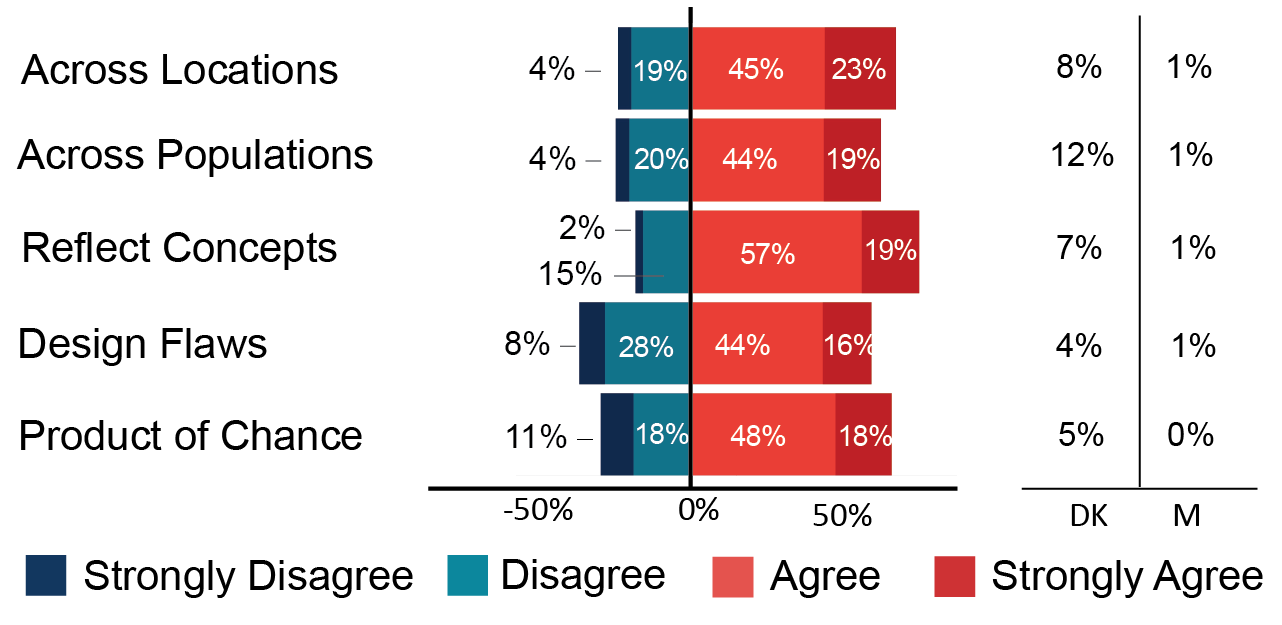
\includegraphics[scale=1]{results/figures/Fig1-Q7-Epistemology.png}
    \caption{Perceptions of the epistemological function of replication studies. Respondents identified the extent to which they agree replication studies can be used to assess the claims or features of past research; `don't know' (DK), and missing (M) responses.}
    \label{fig:Q7-Epistemology}
\end{figure}

%%%%%%%%%%%%%%%%%%%%
\newpage

\begin{figure}[hbt!]
    \centering
    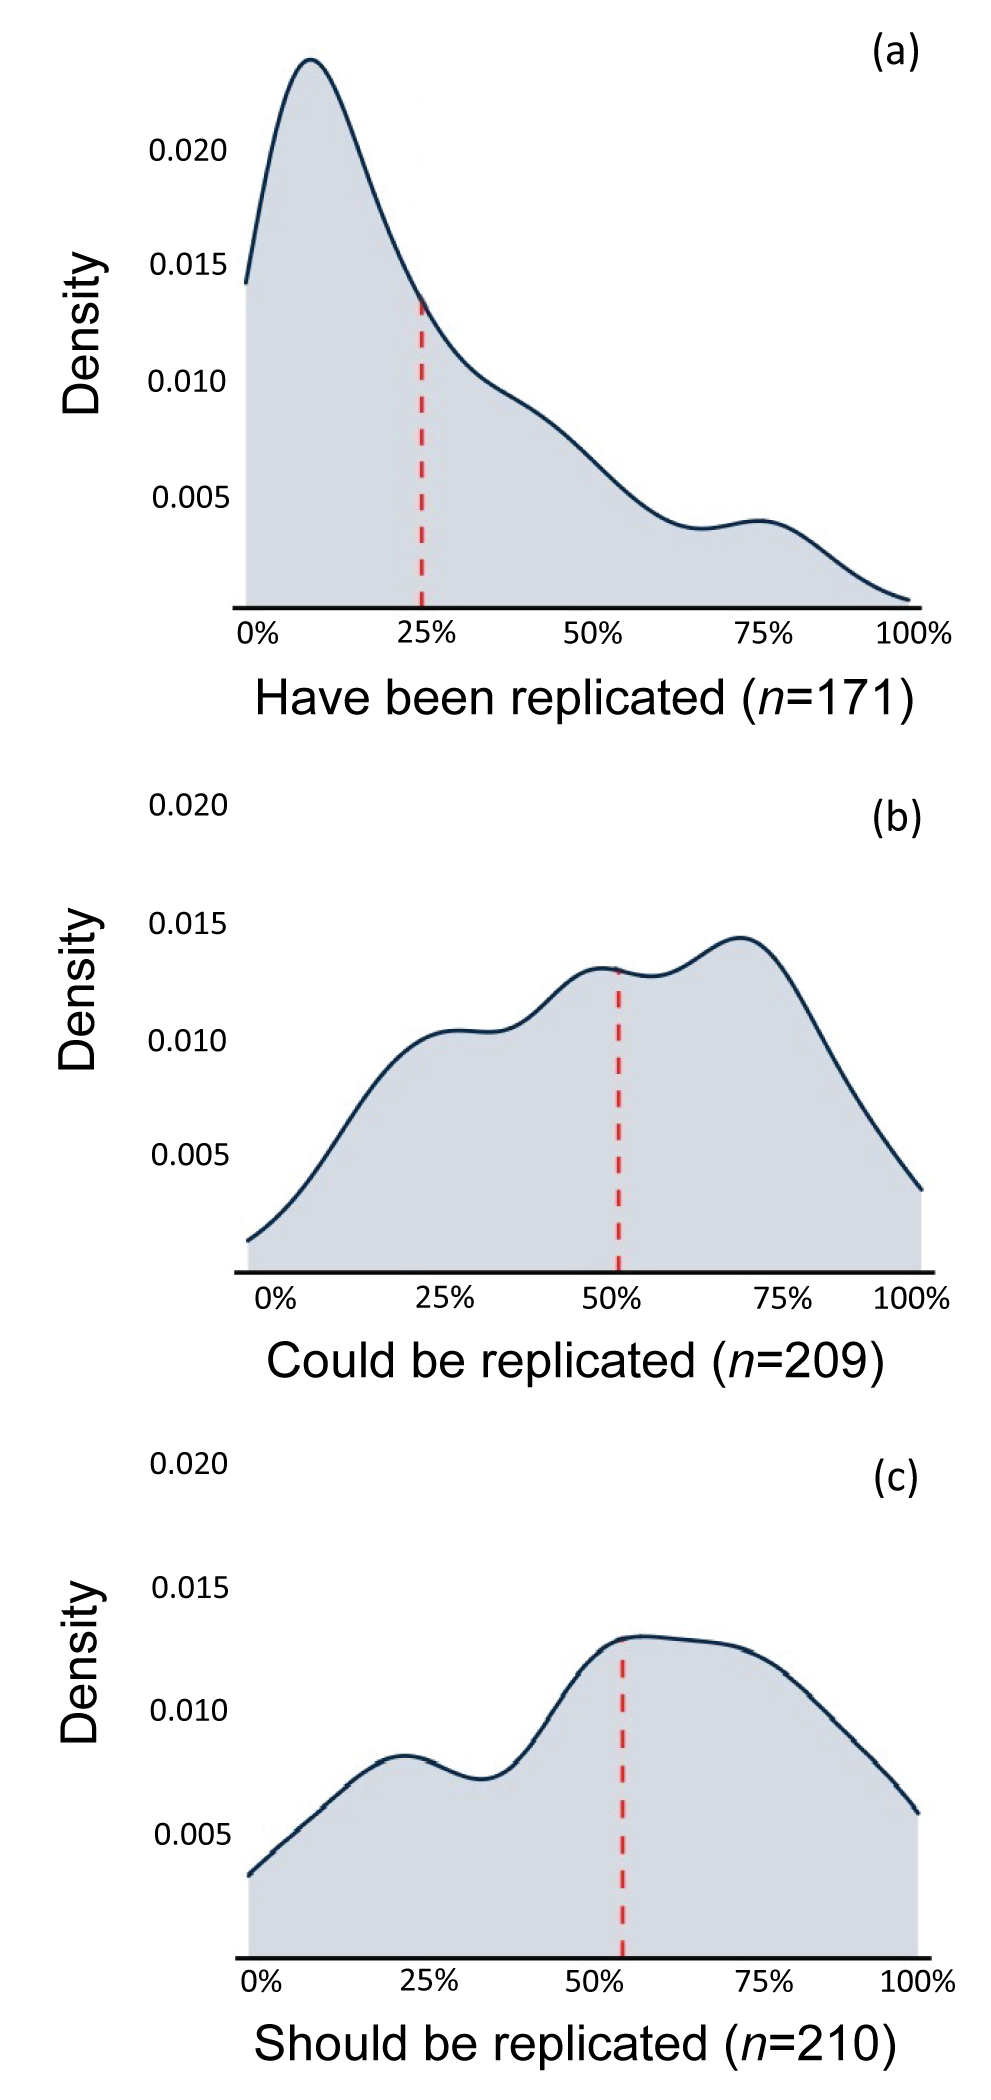
\includegraphics[scale=0.5]{results/figures/Fig2-Q12-HCS.png}
    \caption{Estimates of the percentage of geographic studies that (a) have been replicated, (b) could be replicated, or (c) should be replicated}
    \label{fig:Q12-HCS}
\end{figure}

%%%%%%%%%%%%%%%%%%%%
\newpage

\begin{figure}[hbt!]
    \centering
    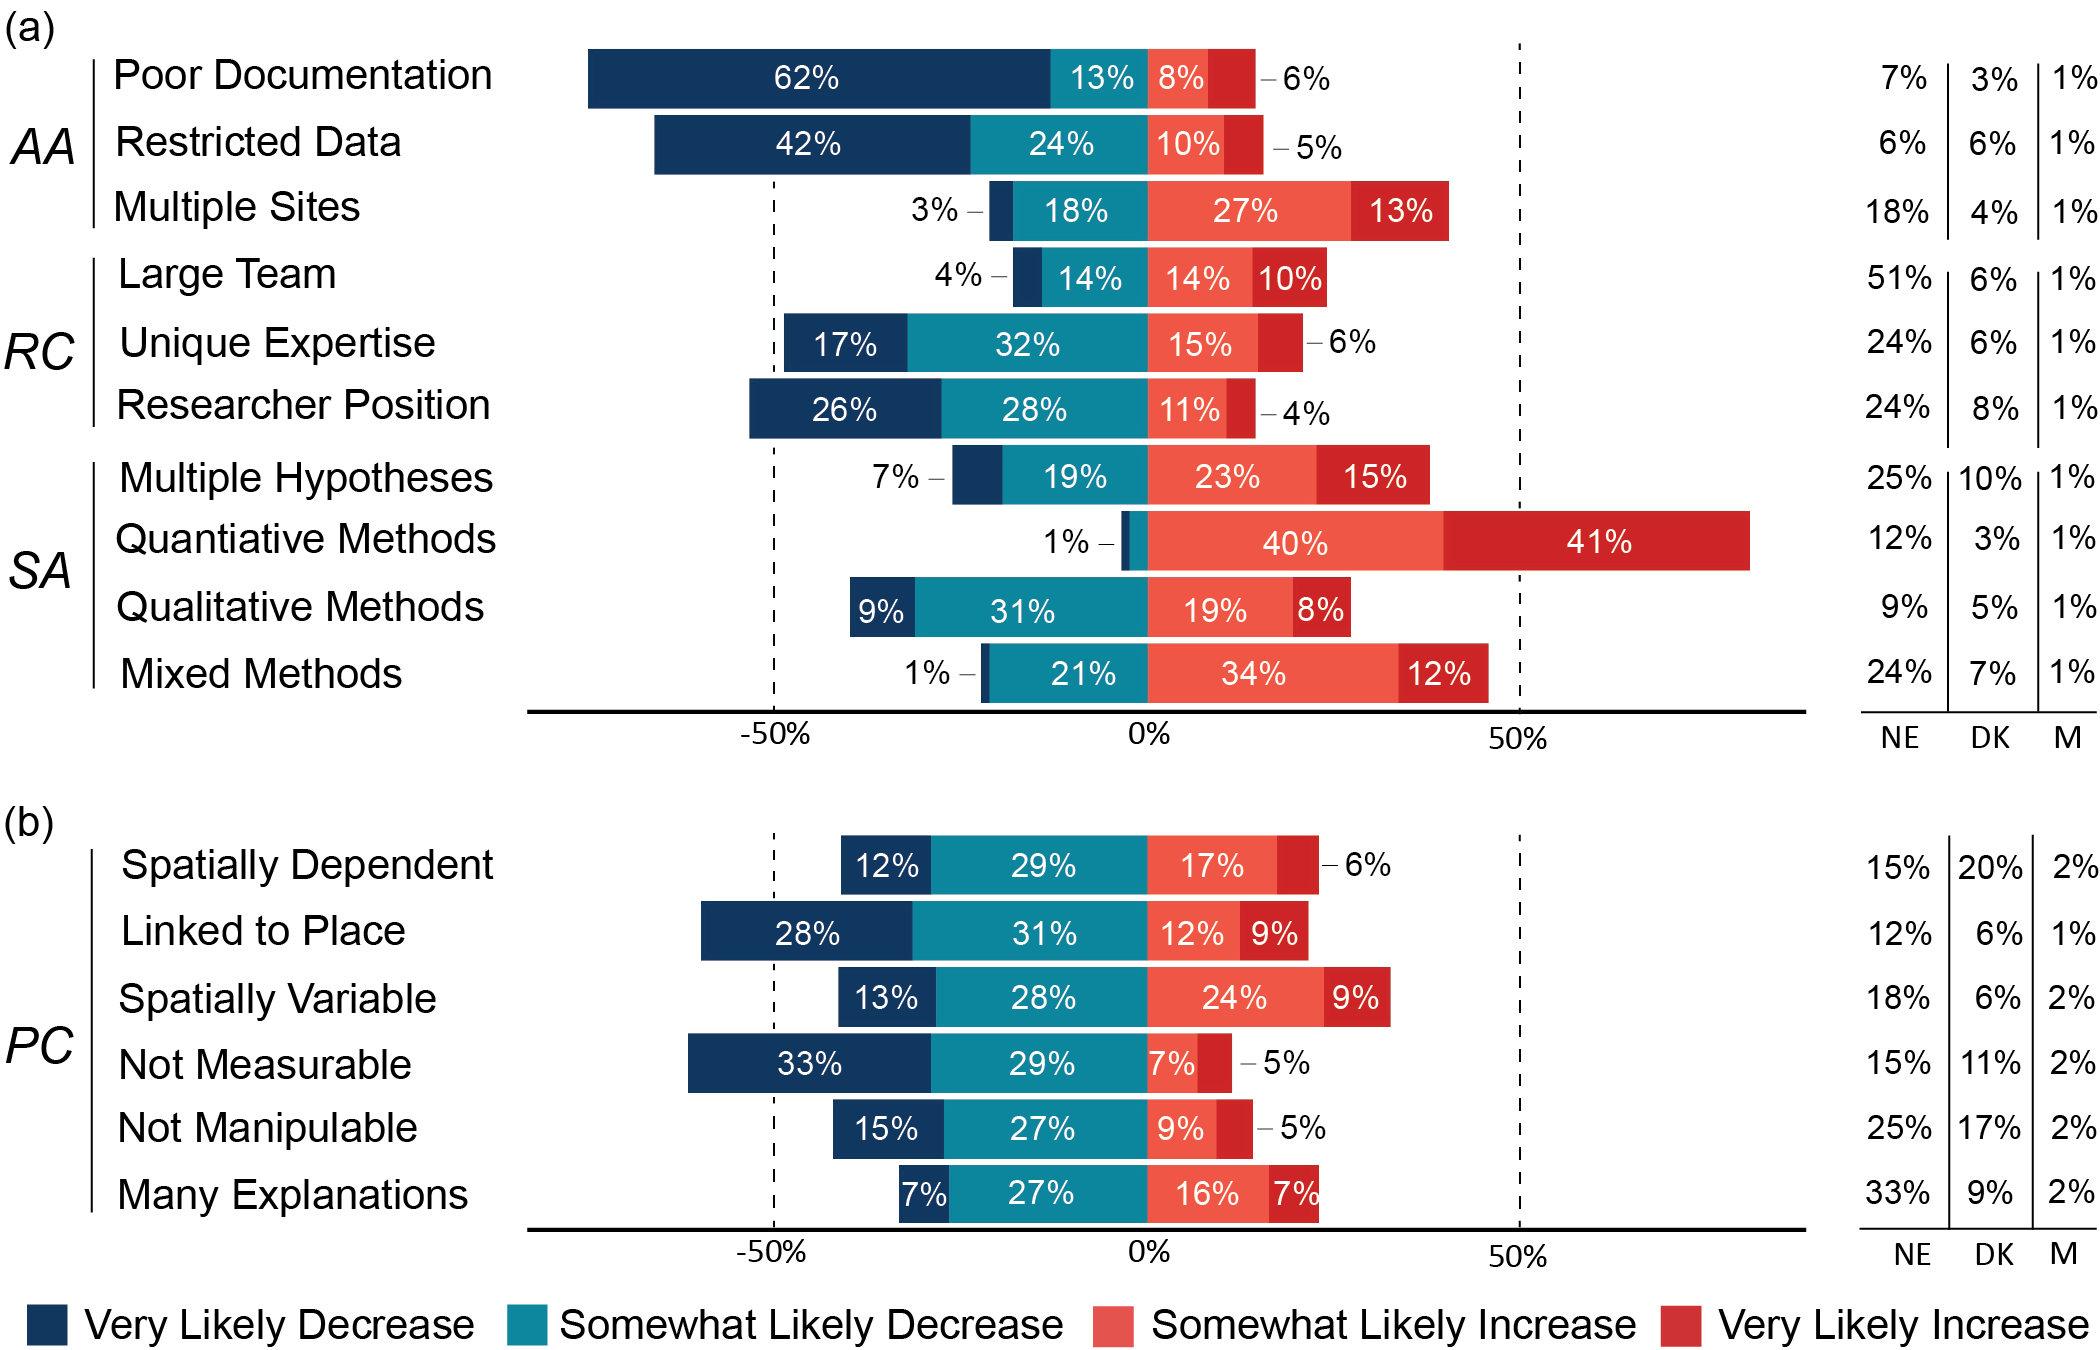
\includegraphics[scale=0.8]{results/figures/Fig3-Q8-10-Chances.png}
    \caption{Factors affecting the chances of replicating a study. Respondents identified (a) how likely study characteristics were to alter the chances of successfully replicating a study and (b) how likely the characteristics of the phenomenon under investigation were to alter the chances of successfully replicating a study in a new location. Acronyms indicate: artifact accessibility (AA), researcher characteristics (RC), study approach (SA), and phenomenon characteristics (PC); and the percentage of no effect (NE), `don't know' (DK), and missing (M) responses.}
    \label{fig:Q8-10-Chances}
\end{figure}

%%%%%%%%%%%%%%%%%%%%
\newpage

\begin{figure}[hbt!]
    \centering
    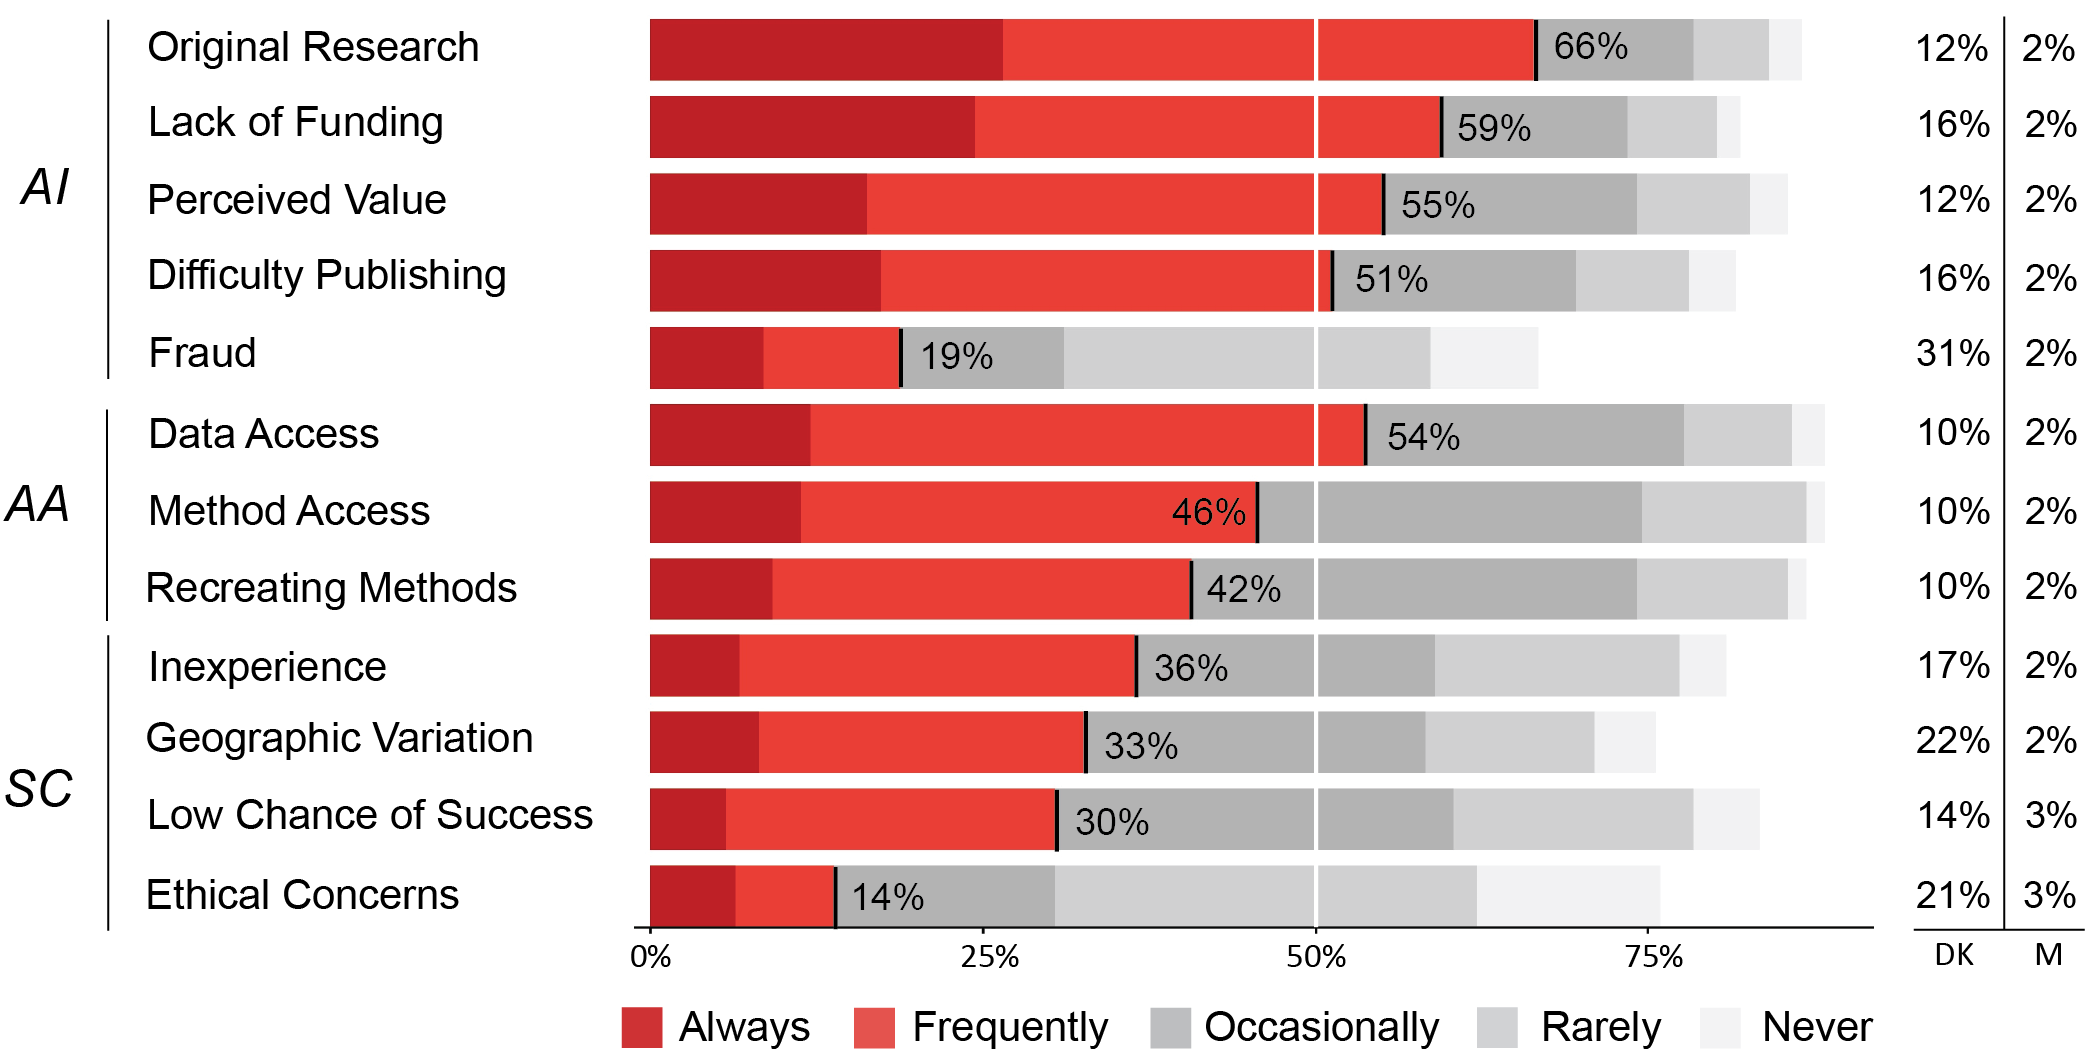
\includegraphics[scale=0.80]{results/figures/Fig4-Q15-Decisions.png}
    \caption{Factors Affecting Researcher Decisions to Undertake Replication Studies. Factors grouped by: Academic Incentives (AA), Artifact Accessibility (AA), Study Characteristics (SC); and the percentage `don't know' (DK) and missing (M) responses.}
    \label{fig:Q15-DecisionFactors}
\end{figure}

%%%%%%%%%%%%%%%%%%%%
\newpage
\noindent PETER KEDRON is an Associate Professor in the School of Geographical Science and Urban Planning and core faculty member in the Spatial Analysis Research Center (SPARC) at Arizona State University, Tempe, AZ, 85283, US. Email: Peter.Kedron@asu.edu. His research interests include spatial analysis, geographic information science, economic geography, and the accumulation of knowledge about geographic phenomena. \\  
  
\noindent JOSEPH HOLLER is an Assistant Professor of Geography at Middlebury College, Middlebury, VT, 05753, US. Email: \\
  
\noindent SARAH BARDIN is a PhD candidate ...

\end{document}